\chapter{Model-Driven Development}
\label{mddchapter}



\section{The Future of Software and Systems Engineering} \label{futureengineering}

\subsection{Managing Complexity Is Not Enough} \label{complexityanddiversity}

This being a software and systems engineering book, we feel duty bound to start with something along the following lines:

\begin{quote}
The theories, methods and tools of software and systems engineering bring a discipline to the development process that enable the increasing complexity of today's systems to be managed in a rigorous and scalable manner.
\end{quote}

This also being a software and systems modelling book, we feel obliged to carry on with something like this:

\begin{quote}
Software and system modelling is the latest step in a continuing trend of increasing abstraction in system development, allowing us to move further away from the low-level implementation-oriented viewpoint towards the high-level problem-oriented viewpoint.
\end{quote}

So is that it? Is modelling the means of coping with the problems of modern software and system development? The anwser to the latter question is an unequivocal "yes!", but not in the way it is currently being applied. The plight facing today's developers is not simply one of complexity (although this is bad enough) - there are many other factors to contend with. This chapter investigates the true nature and needs of modern software and system development, and proposes an approach that is in tune with those needs.

So no, the above soundbites certainly are not "it".

\subsection{Managing Diversity: The New Software Crisis?} \label{diversity}

Before we start to talk about model-driven anything, we need to clarify what the problems are that we're trying to solve. Here are some problems commonly faced by developers today:

\subsubsection{Diverse Domains}

The requirements of large systems often relate to a variety of domains that need to be reconciled by different stakeholders. These requirements may range far and wide, including functional, safety, security and performance considerations. Each domain often has its own specialist approach for dealing with appropriate requirements requirements, but their specialist nature inevitably precludes them from being applied in other domains.

\subsubsection{Diverse Customer Requirements}

The 'one size fits all' approach to software and systems is increasingly inappropriate in today's market. Vendors who offer products that can be tailored to the specific needs of a customer have a strong commercial advantage, but developing products that are truly customisable such that they can meet the demands of a broad customer base is a far from trivial matter. Despite the fact that two products being offered to different customers may share significant functionality, large rewrites and redesign are often required because the functional components of a system are too tightly coupled to allow large scale reuse. In addition, many systems are designed at too lower level of abstraction to yield optimum flexibility.

\subsubsection{Diverse Implementation Technologies}

Systems often need to be deployed across different implementation technologies, each of which have their own requirements and languages. However, the separation between the core functionality and the requirements of the deployment platform is rarely kept clean during the development of the system. It has been recognised that in order to support redeployment (or indeed other customisation such as described above), systems need to be designed at a high level of abstraction; thus software and system modelling has become popular, but these models are rarely complete. Software models in particular seldom get beyond the specification of their behaviour, such that code cannot be completely generated. Even when code is generated, full testing and validation is usually required, and that is a significant chunk of development effort.

\subsubsection{Diverse Tools and Artefact Types}

During the development of a system, a large number of artefacts are created, including requirements specifications, design documentation, design and analysis models, analysis and simulation data and of course the code (for software systems). Unfortunately, these artefacts are often prevented from being truly valuable assets because:
\begin{itemize}
\item they are often created by different incompatible tools or using different languages, some of which may no longer be supported, such that the artefacts become unmaintainable;
\item the forms of artefacts are incompatible, and many are written in informal languages, such that there is no clear way to integrate the information they contain;
\item artefacts such as design models are rarely kept in step with changes to the implementation artefacts such as code, because there is no automatic way to do, vastly reducing their value as assets;
\item the artefacts that are kept up to date, such as code, are often tightly coupled to the integration technology, reducing their value as reusable assets;
\item many artefacts only exist on paper rather than electronic form, so any maintenance or integration tasks has to be manually.
\end{itemize}
This may be fine for one-off stable systems, but systems are rarely built from scratch - they are often based on existing systems, and as such would ideally reuse as much as possible from the baseline system. Similarly, nearly all systems evolve, and code is not always the ideal starting point for managing change.

\vspace{1cm}
\noindent
All the above point to diversity as the new major problem facing developers today. Modelling has certainly helped to manage complexity by raising the level of abstraction, but does not in itself tackle the problem of diversity. One way of tackling it is to try to stem the flow of diversity itself by finding a common language with which developers can model their systems - section \ref{uml} charts one well-known valiant but ultimately doomed attempt at this. The other alternative is to go with the flow and embrace the full multi-coloured tapestry of diversity head-on. This is where true Model-Driven Development (or MDD) differs from common or garden modelling. Simple modelling has the weapon of abstraction to wield, but Model-Driven Development adds the weapon of languages.


% = = = = = = = = = = = = = = = = = = = = = = = = = = = = = = = = = = = = = = =


\section{The Vision of Model-Driven Development} \label{mddvision}

\subsection{Languages are the Future}

Section \ref{diversity} highlighted how diversity lies at the heart of modern system development. Going a step further, we suggest that the challenge really boils down to a diversity of languages:
\begin{itemize}
\item specialists require languages to address the particular facets of the problem that lie within their domain - often within each specialist domain there are numerous languages, with new languages being developed all the time;
\item there are countless implementation languages - some differences are due to the continuing trend of increasing abstraction, some are due to the fact that different paradigms or individual languages are better suited to a particular problem-solution pair than others, and some are simply down to competitive commercial interests;
\item the languages and syntax that capture the artefacts created during the development lifecycle.
\end{itemize}

If a development process limits itself to the application of a fixed set of languages, it will necessarily limit the range of problems that it can address as well as the potential solutions it can provide. Instead, a development process should incorporate the ability to adopt and construct whatever languages provide the best fit. In other words, there should be a shift in emphasis from system development to language development.

One could argue against this by saying that Turing and Church demonstrated that everything can in fact be boiled down to constructs in a very simple language, but this is a theorist's argument. Whilst it is technically feasible, any gain made in widening the applicability of a language to different domains will be at the expense of the richness of the language that makes it so suitable for a particular domain (section \ref{uml} describes some of the pitfalls of this approach in more detail). However, in a very real sense, the concept of a single small underlying language provides the basis for realising Model-Driven Development. This is the domain of metamodelling, and is the topic of Chapter \ref{metamodellingChapter}.

It is important to clarify what we mean by the term 'language' here. Section \ref{syntaxsemantics} describes the features and components of languages in detail, but there are two important points to make here in the context of Model-Driven Development. Firstly, in order to be useful, a language should be a precise and unambiguous formalism - in other words, there should be clear rules which dictate what does and does not constitute a valid application of the language. Without this, any form of rigourous analysis, testing or transformation becomes impossible. Secondly, a language must have meaning (also known as semantics) as well as form (also known as syntax). Any formalism which has no meaning is a notation rather than a language. Notations have their part to play in MDD, but it is important to realise that by definition, in order to have meaningful models, the language in which they are described must have a semantics. In addition, just as with syntax, in order to be useful in an MDD context, the semantics must be precisely defined. These points may seem obvious, but in fact, many formalisms which are currently used for system and software modelling can really only be described as notations rather than languages - this severely limits the potential power that these formalisms can yield in the MDD world.


%Productivity can be increased because engineers and domain experts can speak in the languages they understand, and both the problem space and solution space are opened up to their full extent. [This approach could potentially offer a layer/ paradigm shift above OO programming that could have major implications in terms of productivity, etc to industry. (Andy e-mail)]


\subsection{Language Integration}

%language islands
%proof: lots of dsl's - argument that there only not more of them because language islands don't work

\subsection{Requirements of MDD} \label{mddreq}
%Problem-driven not technology-driven (James)
%Customers: industrial-based systems and software engineers


% = = = = = = = = = = = = = = = = = = = = = = = = = = = = = = = = = = = = = = =


\section{Current State of Model-Driven Development} \label{mda2mdd}

\subsection{The Unified Modelling Language} \label{uml}

%Trying to have a single homogenous language doomed

%Books such as [] implicitly suggest that a broad range of problems can be solved by a set of languages X, Y and Z (UML, OOA, Booch...). Having said this, the inability of languages such as UML (in its vanilla form) to support tasks such as the engineering of real-time systems, for example, has led to "real-time" extensions to that language via profiles (we shall avoid discussing the limitations of profiles as a language definition mechanism at this stage). But if one is to examine the number of types of requirements faced by real-time systems developers, it is impossible for one language however well designed to anticipate them all. Moreover, the act of trying to design a language which anticipates all possible uses invariably gives rise to a language which is large, difficult to understand and difficult to apply. (This claim is reinforced in the context of real-time systems when one examines the literature which introduces new mechanisms week by week catering for new types of requirements). - James' paper

%Need to outline benefits as well as pitfalls - single language is easier to roll out across developers etc. (Andy)

Modelling has been used in software engineering since its inception, but most methodologies proposed over the years have included their own particular modelling notation and tools, which made model interchange difficult. This invariably led to a situation where software developers were locked into a particular tool vendor that supported a particular methodology \cite{umllrm}. In the nineties, after an influx of object-oriented methodologies such as Schlaer-Mellor \cite{schlaermellor}, Coad-Yourdon \cite{coadyourdon} and OMT \cite{omt}, the Object Management Group \cite{omg} (OMG) instigated a drive to unify the variety of modelling notations (rather than the methodologies), which were seen to share a lot of common concepts.

The result was the Unified Modelling Language (UML)\cite{umlspec}, which was adopted in November 1997. UML consists of a number of different notations that allow different views of a software system to be modelled at different stages of the development lifecycle. Both static and dynamic aspects of a system can be captured, and facilities are also provided to enable model management and limited extensibility (described in more detail in section \ref{???}. A textual constraint language (OCL) is included to allow the state space represented by a model to be further constrained in ways that are too complex to be captured by the graphical notations alone. The UML views and notations are summarised in Table \ref{tableuml}.

\begin{table}[htb]
\begin{center}
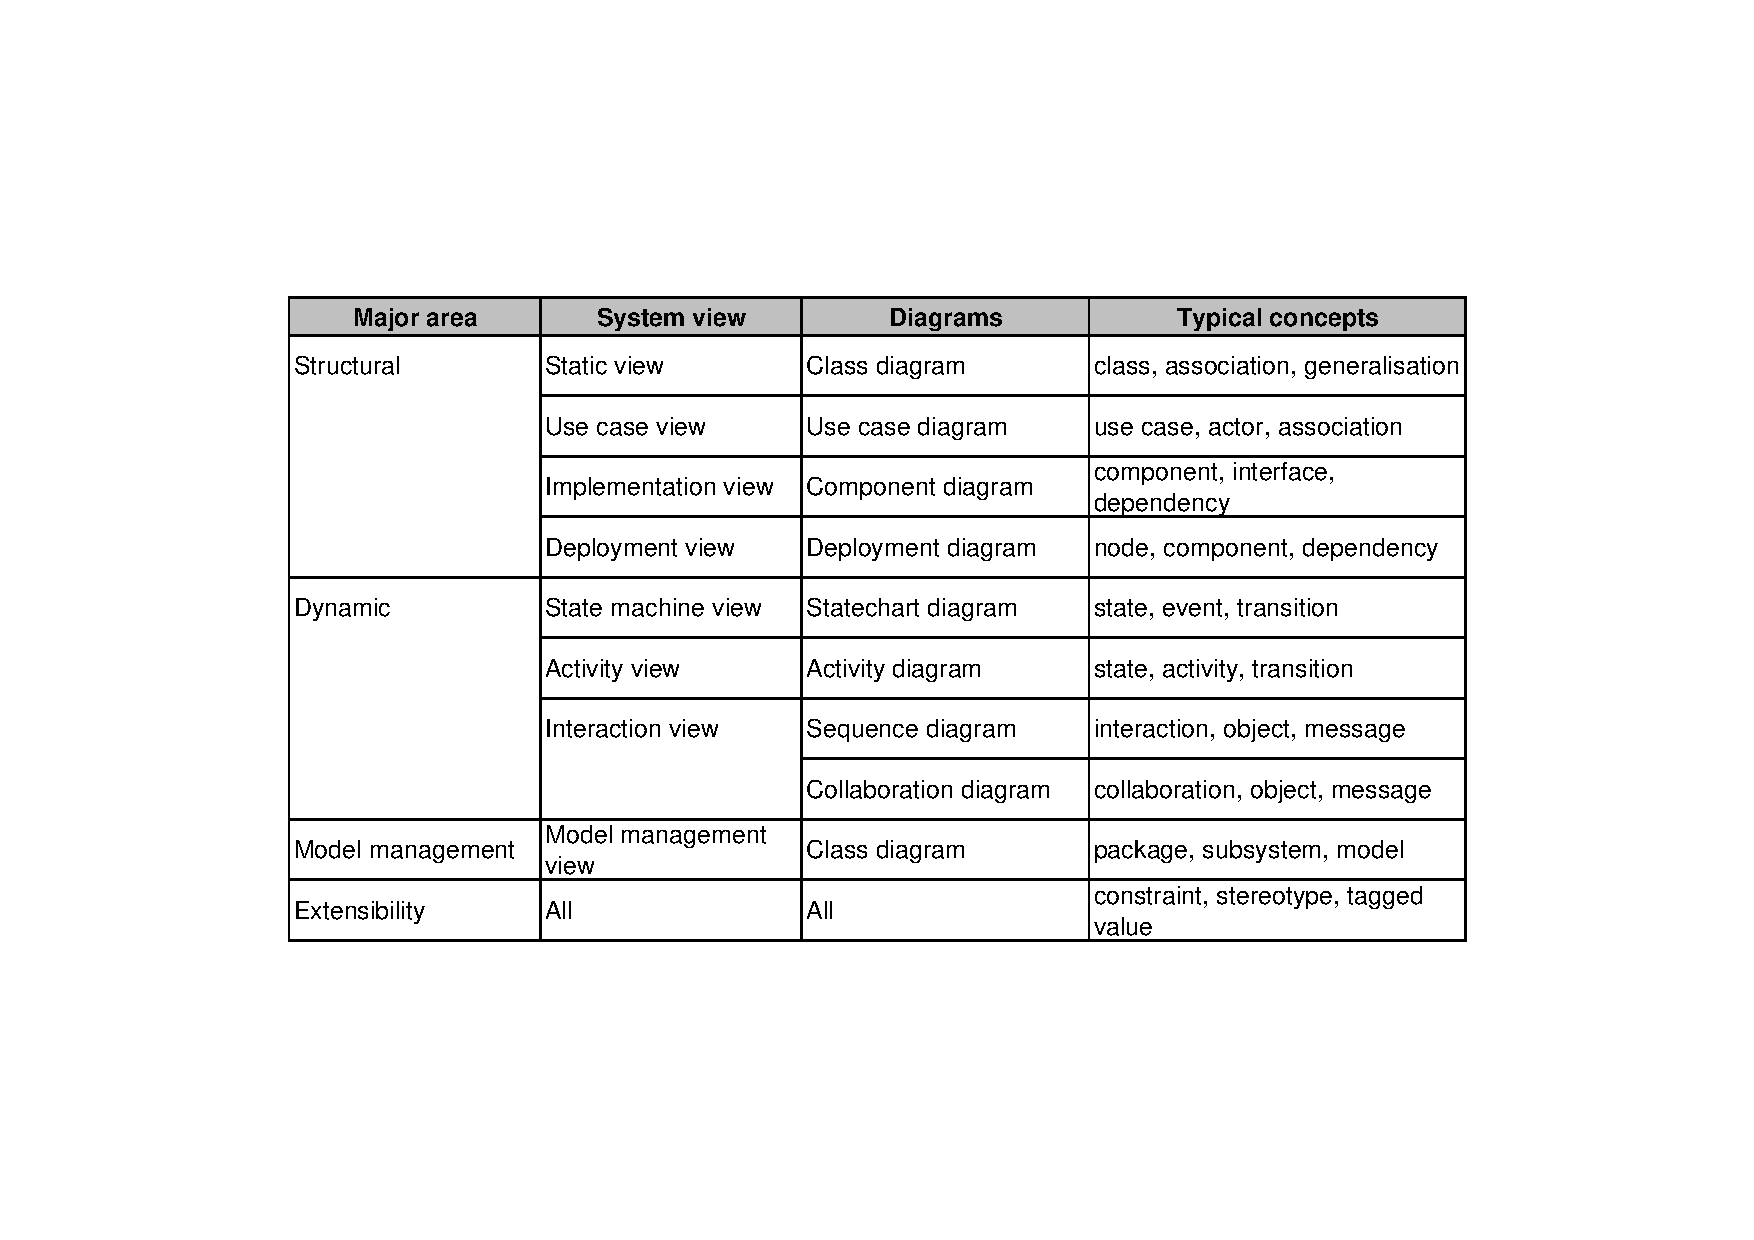
\includegraphics[width=14.5cm]{ModelDrivenDevelopment/figures/tableuml.pdf}
\caption{\textbf{UML Views an Diagrams.} \em{Based on \cite{umllrm}.}}
\label{tableuml}
\end{center}
\end{table}

UML has been well-received and is now the \emph{de facto} software modelling language, but it is not without its shortcomings. The three main areas for concern with UML 1.x, which have led to the development of UML 2.0 and MDA, are listed below and described in detail in the remainder of this section:
\begin{itemize}
\item the definition of the language itself is incomplete, imprecise and incoherent;
\item the language is not flexible enough to support the wide range of potential domains;
\item it is not executable.
\end{itemize}

\subsubsection*{Imprecise semantics}

Section \ref{model} explained the importance of unambiguous models within engineering disciplines, and that in order to achieve this, modelling languages must have a precise semantics. The specification for UML 1.x\cite{umlspec} falls some way short of this - whilst its syntax is mostly well specified, the semantics of those syntactic elements is either missing or provided informally using English. This has led to a situation where, as of version 1.3, no tool could claim to UML compliant \cite{pumlrfi}. This in turn has inhibited model interchange between tools, leading back to the situation of vendor lock-in. In addition, as explained earlier, models written in such an informally specified language are open to misinterpretation, a potentially dangerous or expensive problem. Whilst a major revision of UML will be released soon, draft versions of the UML 2.0 standard do not indicate major improvements with regard to semantics.

\subsubsection*{Limited scope and flexibility}

UML has been successfully applied across the software development community, and it is increasingly being applied to non-software domains such as systems engineering\cite{umlse}, and specialised software domains such as real time and high integrity systems. The diverse modelling requirements that this widespread use brings makes defining what a unified modelling language should be a considerable problem. Early attempts to enhance UML to support new requirements adopted a 'mud-packing' approach\cite{kobryn}, which involved making direct amendments to the monolithic definition of UML itself. This resulted in a language that became increasingly large, unwieldy to use, incomprehensible, and difficult to maintain and test for consistency.

In order to overcome these problems, UML was refactored from a one-size-fits-all modelling language into a family of languages. The foundation of the UML family is a stable core UML metamodel, consisting of minimal modelling concepts that are supported by all family members. Each dialect of UML consists of the UML core metamodel and one or more extensions to the core known as `profiles'. The UML 1.4 profile mechanism is quite straightforward to apply, but is limited as it is based upon constraining existing language constructs rather then modifying or adding new language constructs. The profile mechanism offered by UML 2.0 promises to be more powerful, allowing direct extensions to the language constructs - this is obviously an important step forward. However, it would be naive to think that every possible domain could be modelled using a profile of UML. If nothing else, the UML core is still fundamentally object-oriented, which is quite a problem for non OO domains. Thus in some cases, it is necessary to define modelling languages that are quite independent of UML. How models written in these seemingly disparate languages are integrated into a unified process is the subject of MDA (see section \ref{mdavision}).

\subsubsection*{Non-executability}

*** TO BE FINISHED ***

%action semantics
%executable UML

\subsection{MDA}
%PIMs to PSMs too limited
%MOF not powerful enough
%Architecture not flexible enough
%Too driven by tool-vendors - vaguely defined marketing banner that they can flog their products under

MDA is an ambitious vision that could change the way software is developed in the future. However, there are some limitations to MDA that need to be considered:
\begin{itemize}
\item MDA does not specify the way in which mappings should be realised. A true Model Driven Software Development process would realise mappings as models, as this would bring all the benefits of modeling and allow similar tools to be applied to mappings as other models. It would also allow mappings themselves to be transformed \cite{bezivinmda}.
\item MDA is too fixed on the notion of \emph{platform}. The answer to what constitutes a \emph{platform} is unclear at best - the transition from the most abstract model of a system to the most refined model may include several stages of models, each which could considered Platform Specific when compared to the previous stage, or Platform Independent when compared to the following stage. Also, mapping models or language models as well as system models may be transformed - here the notion of platform makes less sense. Instead, the broader notion of Model Driven Software Development is just concerned with models and mappings.
\item The four layer metamodel architecture of Figure \ref{figmetamodelarch} is quite inflexible, because it arbitrarily limits the number of levels of instantiation \cite{panhorrocks}, enforces a type distinction between models at different layers and does not support the modeling of the instantiation relationship (since they exist outside of all the levels). These and other architectural issues are detailed in section \ref{archprobs}.
\end{itemize}

%Andy Key that we get across that MDD is not just about PIM to PSM mappings it is about being able to capture all aspects of the systems development process etc in a unified way, and all the benefits that brings to developers.

\subsection{QVT}


% = = = = = = = = = = = = = = = = = = = = = = = = = = = = = = = = = = = = = = =


\section{Conclusion}
%Complexity AND diversity
%Languages are the new OO
%Mappings
%Integration of artefacts written in different languages - next chapter introduces a means of doing this
%Introduction to rest of book





%*** Andy's Metamodelling chapter ***
%2.0: The previous chapter described how model-driven development is fundamentally based on the use of modelling languages to capture and relate different aspects of the problem domain. These languages may be general purpose languages like UML or domain specific languages such as XML.
%2.1.4: In the real world, modelling languages do not exist in isolation. They will always be related to other languages.
